\chapter{Optimización del modelo: Algoritmos Genéticos}

\section{Introducción, operadores e implementación}

Para optimizar el modelo, decidimos optar por usar un modelo basado en algoritmos genéticos, debido a la flexibilidad que ofrecen, ya que ofrecen la posibilidad de tener una alta diversidad en la población y la capacidad de producir fuertes optimizaciones en el modelo, introduciendo una búsqueda local durante el proceso de optimización, realizando lo que se conoce como \textit{algoritmo memético}.

Esto se pensó así ya que podríamos hacer fácilmente operadores para la mutación de las soluciones, como podía ser cambiar el orden en el que se cursaban las asignaturas. Es decir, si las dos primeras horas son horas de prácticas y las dos siguientes son horas de teoría, se intercambiaban estas horas, como se ven en la \hyperref[mut1]{Figura \ref*{mut1}}.

\begin{figure}[H]
\centering
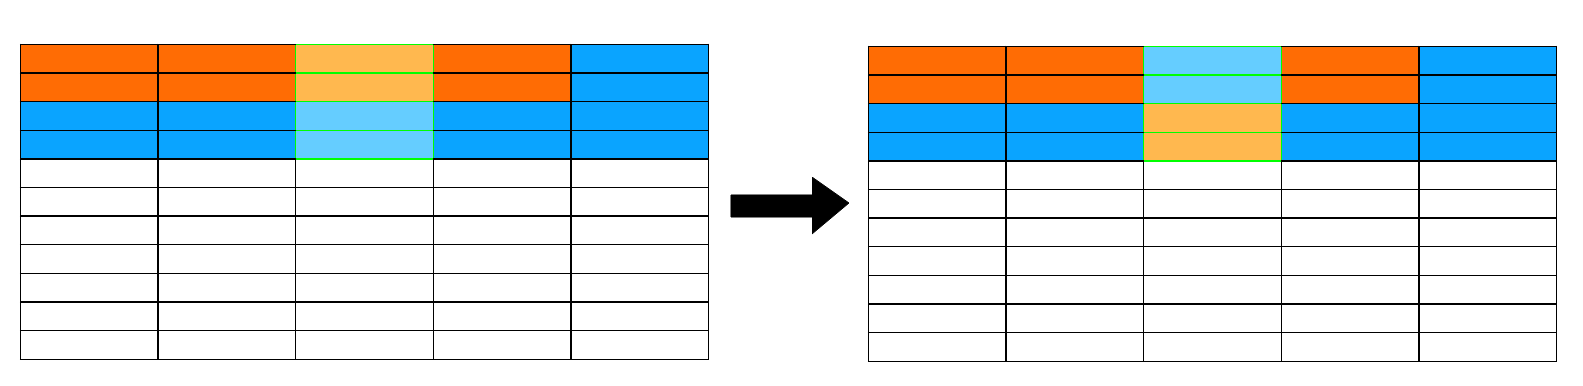
\includegraphics[width=1\textwidth]{img/mut1}
\caption{Operador de mutación.}
\label{mut1}
\end{figure}

En esta imagen podemos ver cómo las casillas de la estructura en un color más claro y remarcadas en verde, cambian de posición y generan una nueva estructura, con una nueva solución. 

También se pensaron varios operadores de cruce:

\begin{enumerate}
	\item A partir de dos padres, generar dos nuevas soluciones intercambiando dos grupos completos. Por ejemplo, intercambiar los cursos 3ºA de ambos padres y generar dos nuevos hijos.
	\item A partir de dos padres, intercambiar dos grupos completos. En este caso, la diversidad cambia poco y hay que hacer un operador de mutación más agresivo, o probar varias técnicas de mutación.
\end{enumerate}

Además de esto, se usó como operador de selección una selección por torneo clásica, introduciendo a partir del operador de cruce, sólo las mejores soluciones.

Para el desarrollo del algoritmo genético, se usó el framework de Python \textit{DEAP}, \textit{Distributed Evolutionary Algorithms in Python}. Este framework permite que solo definiendo el tipo de solución, operador de cruce y mutación, podemos tener un algoritmo genético en breve tiempo, ya que tiene implementadas una gran cantidad de operaciones, al igual que nos permite modificar parámetros del algoritmo de forma muy sencilla. 

Como desventaja tiene que no es una librería que tenga el paralelismo de forma nativa, pero en su documentación (\url{http://deap.readthedocs.io/en/master/}), podemos encontrar guías para paralelizar el algoritmo.

\section{Problemas del algoritmo genético}

La idea de utilizar un algoritmo genético para optimizar la generación de horarios fue algo que se abandonó pronto por varias razones:

\begin{enumerate}
	\item Consumo de recursos: el aumento de los recursos que necesitaba el algoritmo creció muchísimo respecto a la versión del algoritmo Greedy, debido al mantenimiento de la población, el coste computacional de las operaciones de cruce y mutación, etc.

	Esto también se debe a que al realizar las operaciones de cruce y mutación, había que ``parar'' el algoritmo para arreglar la solución, ya que había colisiones en las aulas, algunos grupos se quedaban sin aula, etc. lo que aumentaba muchísimo el tiempo de cómputo del algoritmo, lo que nos lleva a la siguiente razón.

	\item Tiempo de cómputo: para obtener resultados que tuvieran un mínimo de calidad, había que ejecutar un gran número de iteraciones. Esto, hace que el algoritmo pierda el dinamismo que tenía ejecutando el algoritmo Greedy, que era ejecutar el algoritmo y tener de forma prácticamente instantánea un resultado de calidad. 

	Con el algoritmo genético, había que dejar bastante tiempo la máquina ejecutando, y aun así, apenas mejoraba la calidad de los resultados.

	\item Problemas de los operadores de cruce: los problemas de colisiones en las aulas que aparecían de ejecutar los algoritmos de cruce, hacen empeorar mucho el algoritmo, tanto que casi parece contraproducente. 

	Ha habido ocasiones que obviando el operador de cruce y ejecutando sólo el operador de mutación, se han obtenido mejores resultados.
\end{enumerate}

Estas son las razones principales por las que se abandonó el algoritmo genético además de que, por todas estas razones, el algoritmo ya necesitaba unos requisitos hardware mucho mayores que en la primera versión, cosa que hace que ejecutar el algoritmo y tener una solución en un tiempo viable, sea impensable.